\section{Model Specification} 
        \subsection{Pictorial Depiction}
            Chain drives and shafts combined have been modelled as thick round gears.
            \begin{figure}[hbt!]
                \centering
                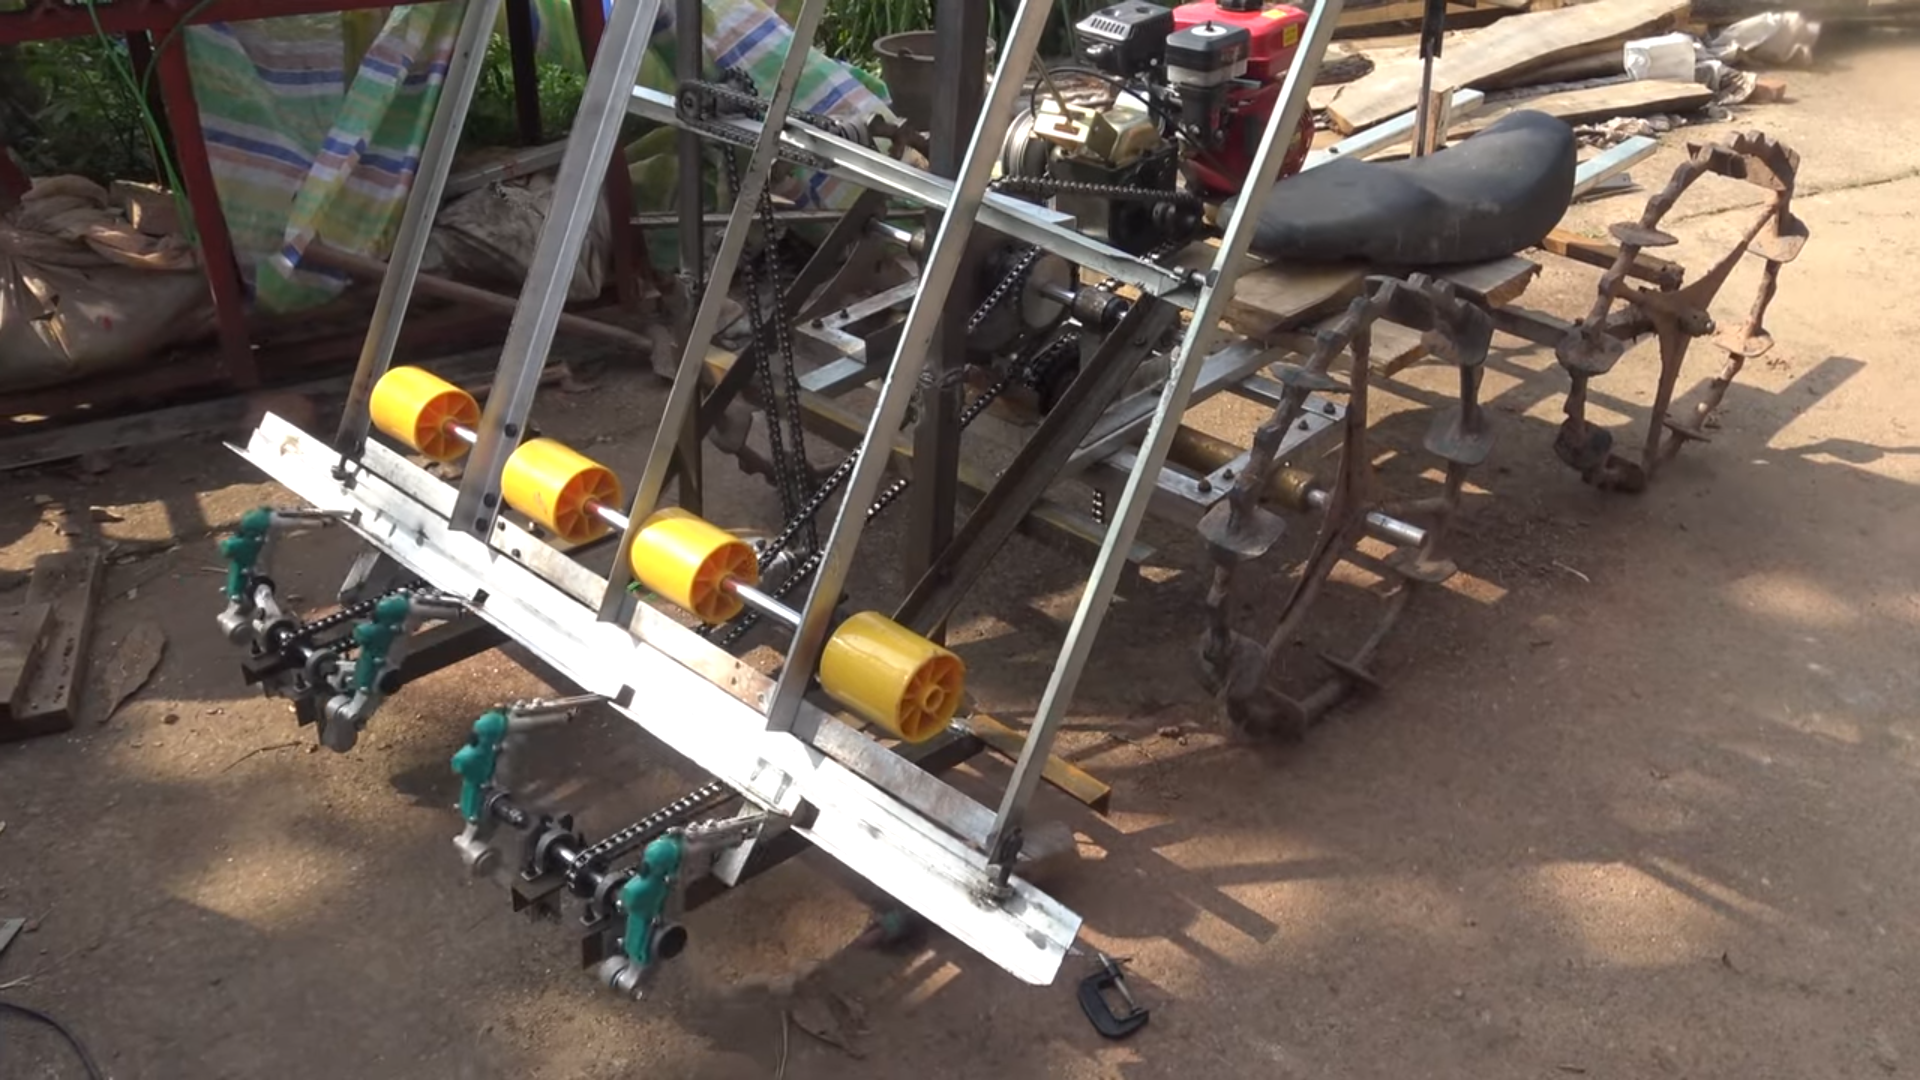
\includegraphics[width=0.9\columnwidth]{Images/Actual_mechanism.png}
                \caption{Actual mechanism}
                \label{fig:actual_mechanism}
            \end{figure}

            \begin{figure}[hbt!]
                \centering
                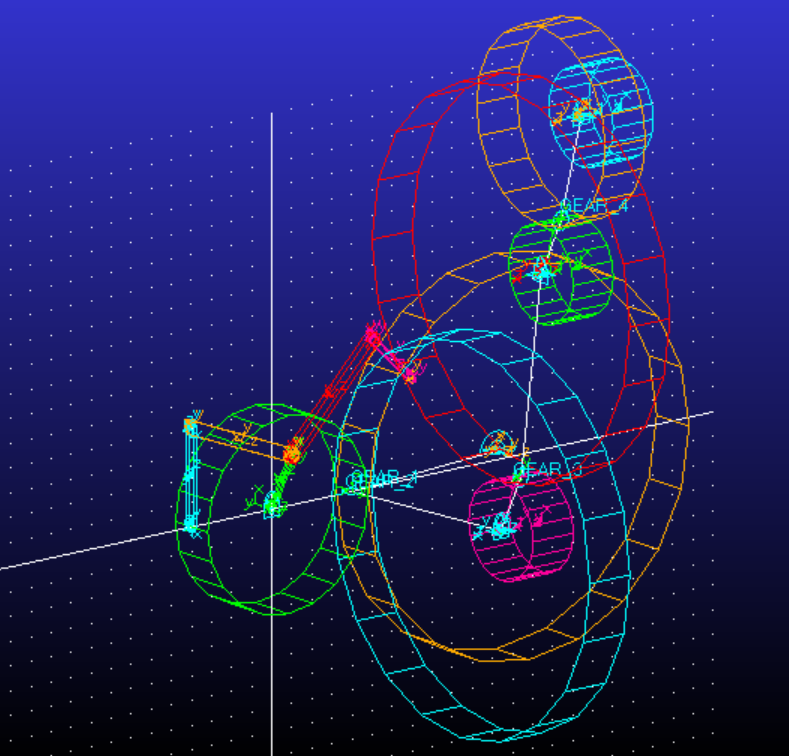
\includegraphics[width=0.9\columnwidth]{Images/Model_mechanism.png}
                \caption{Model mechanism}
                \label{fig:model_mechanism}
            \end{figure}

            \begin{figure}[hbt!]
                \centering
                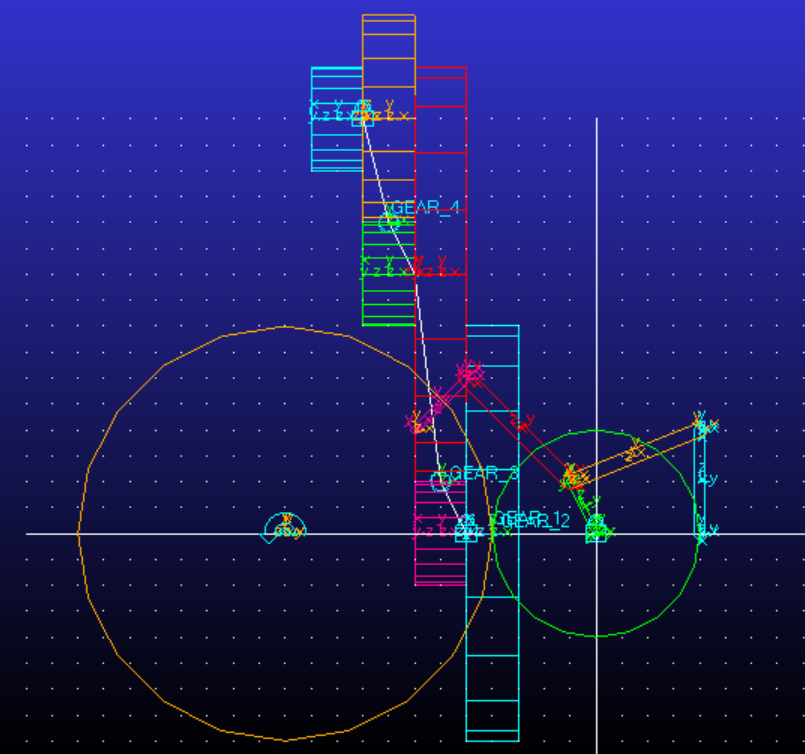
\includegraphics[width=0.9\columnwidth]{Images/Model_fv.png}
                \caption{Front View of Model mechanism}
                \label{fig:model_fv}
            \end{figure}

        \subsection{Geometry and Material}
            \subsubsection{Dimensions of every component}
                All geometrical details required to create the model. These are indicated in figures 4-16.

                \begin{figure}[hbt!]
                    \centering
                    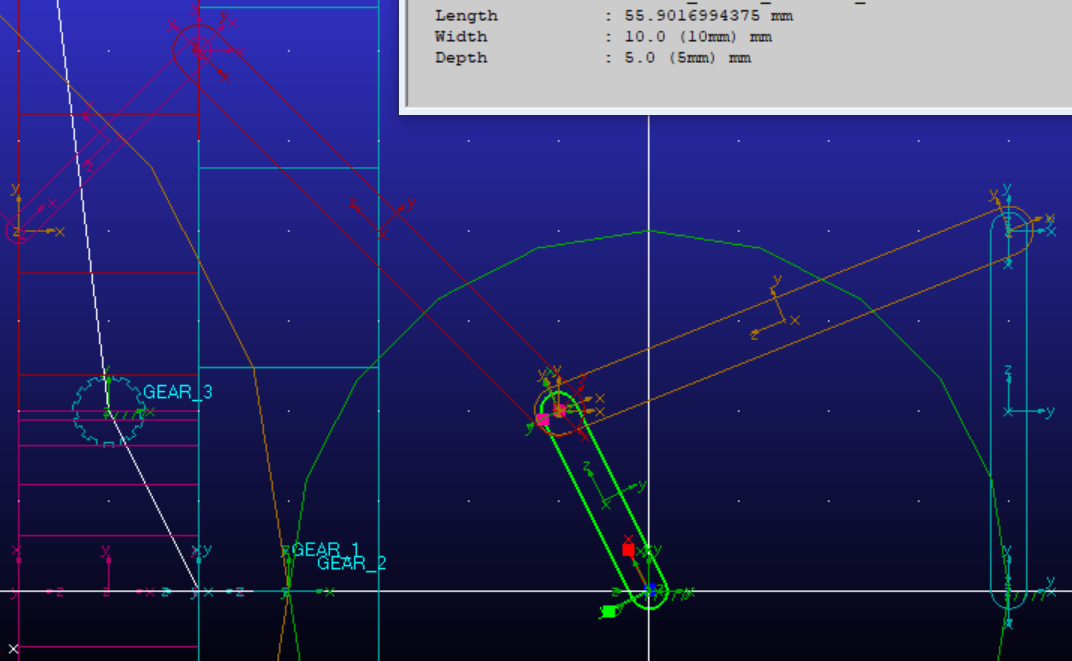
\includegraphics[width=0.9\columnwidth]{Images/dim8.png}
                    \caption{Dimensions of Part 8}
                    \label{fig:dim8}
                \end{figure}

                \begin{figure}[hbt!]
                    \centering
                    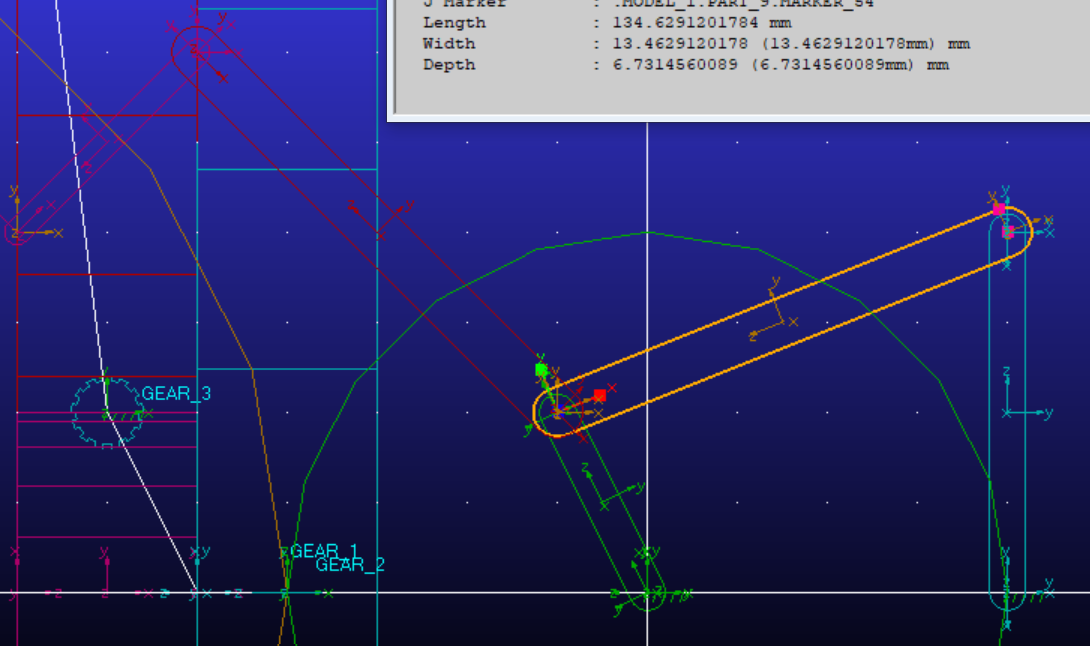
\includegraphics[width=0.9\columnwidth]{Images/dim9.png}
                    \caption{Dimensions of Part 9}
                    \label{fig:dim9}
                \end{figure}

                \begin{figure}[hbt!]
                    \centering
                    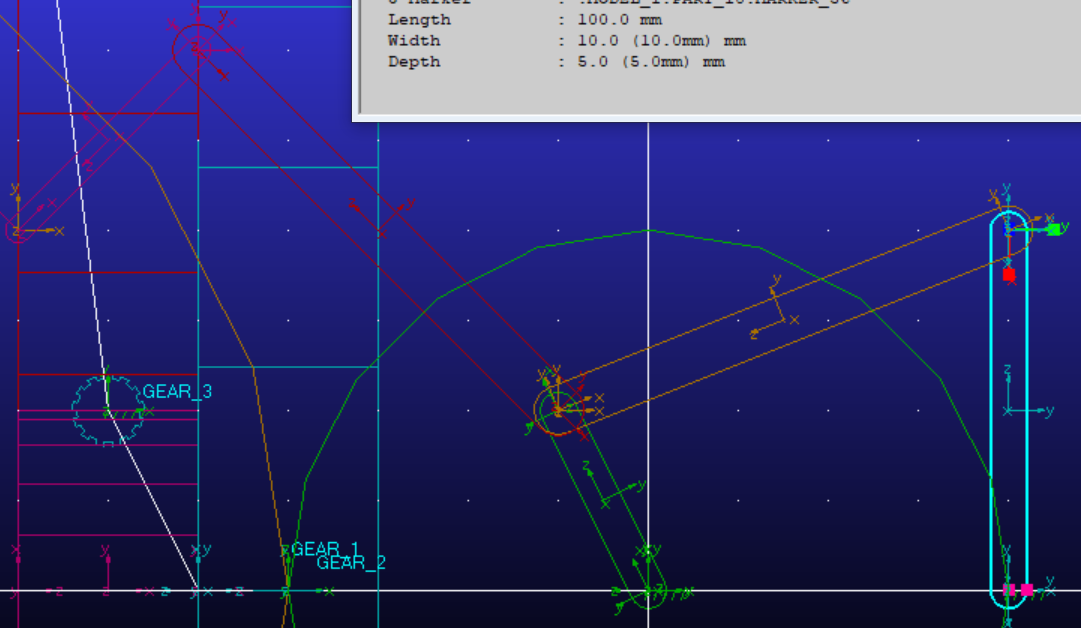
\includegraphics[width=0.9\columnwidth]{Images/dim10.png}
                    \caption{Dimensions of Part 10}
                    \label{fig:dim10}
                \end{figure}

                \begin{figure}[hbt!]
                    \centering
                    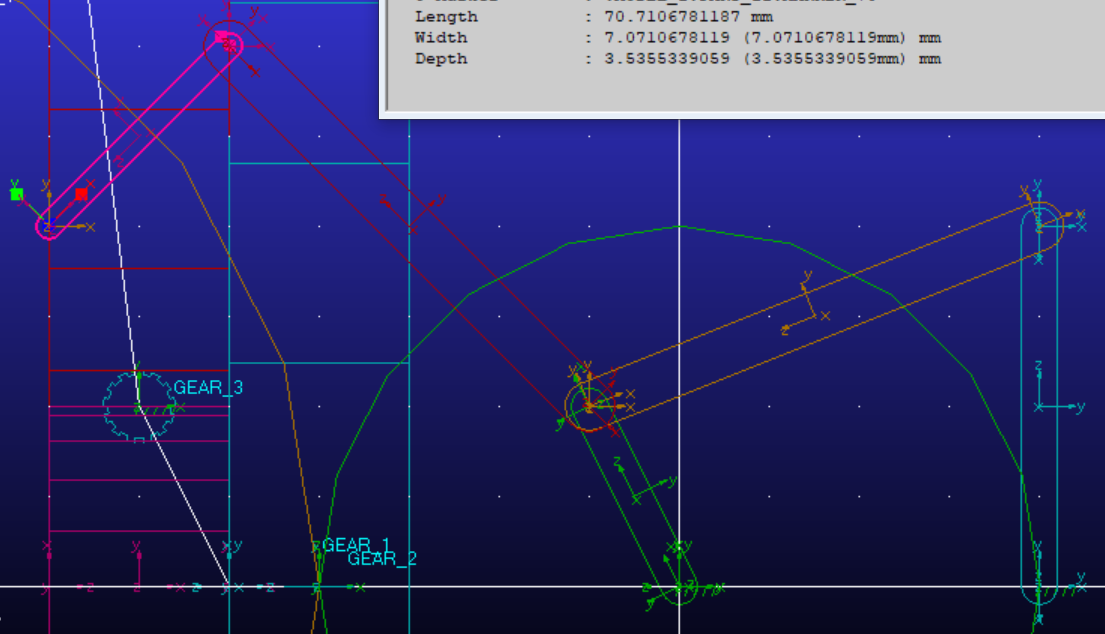
\includegraphics[width=0.9\columnwidth]{Images/dim11.png}
                    \caption{Dimensions of Part 11}
                    \label{fig:dim11}
                \end{figure}

                \begin{figure}[hbt!]
                    \centering
                    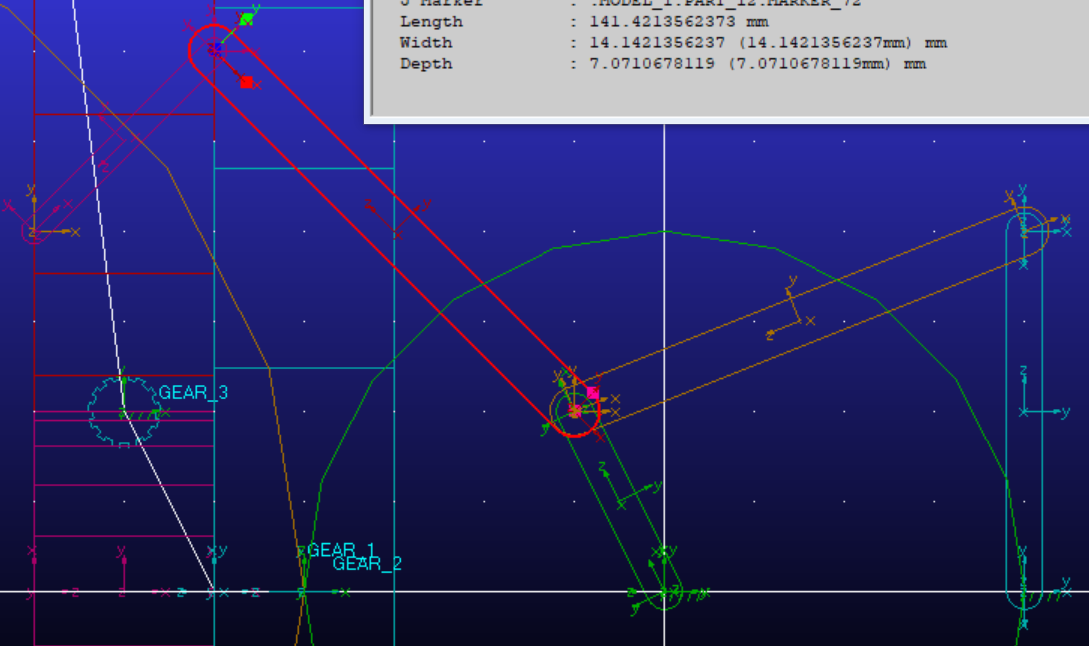
\includegraphics[width=0.9\columnwidth]{Images/dim12.png}
                    \caption{Dimensions of Part 12}
                    \label{fig:dim12}
                \end{figure}

                \begin{figure}[hbt!]
                    \centering
                    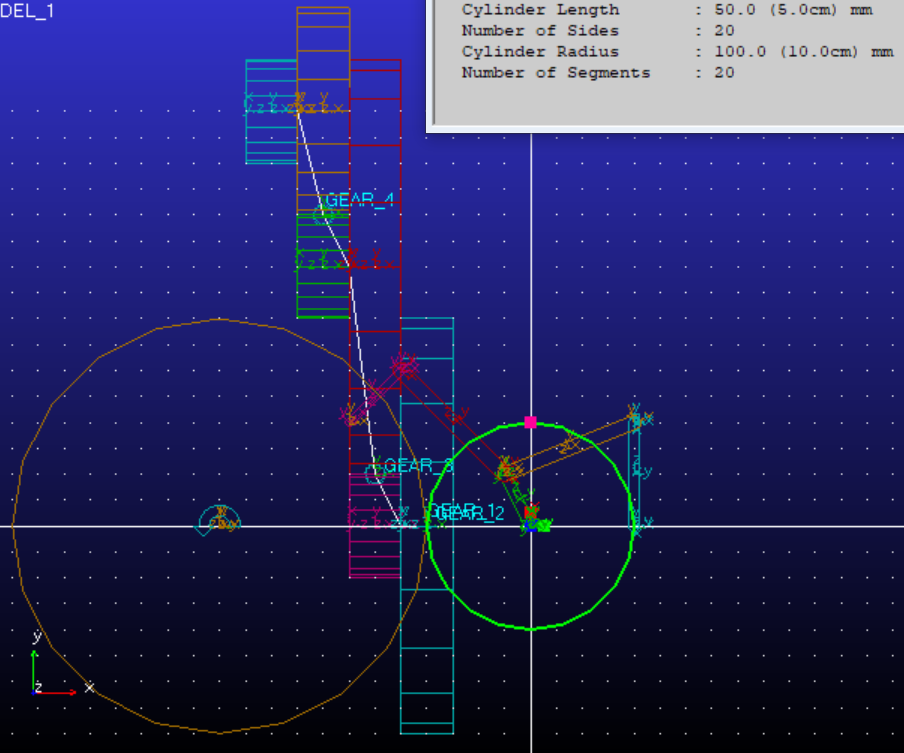
\includegraphics[width=0.9\columnwidth]{Images/dim13.png}
                    \caption{Dimensions of Part 13}
                    \label{fig:dim13}
                \end{figure}

                \begin{figure}[hbt!]
                    \centering
                    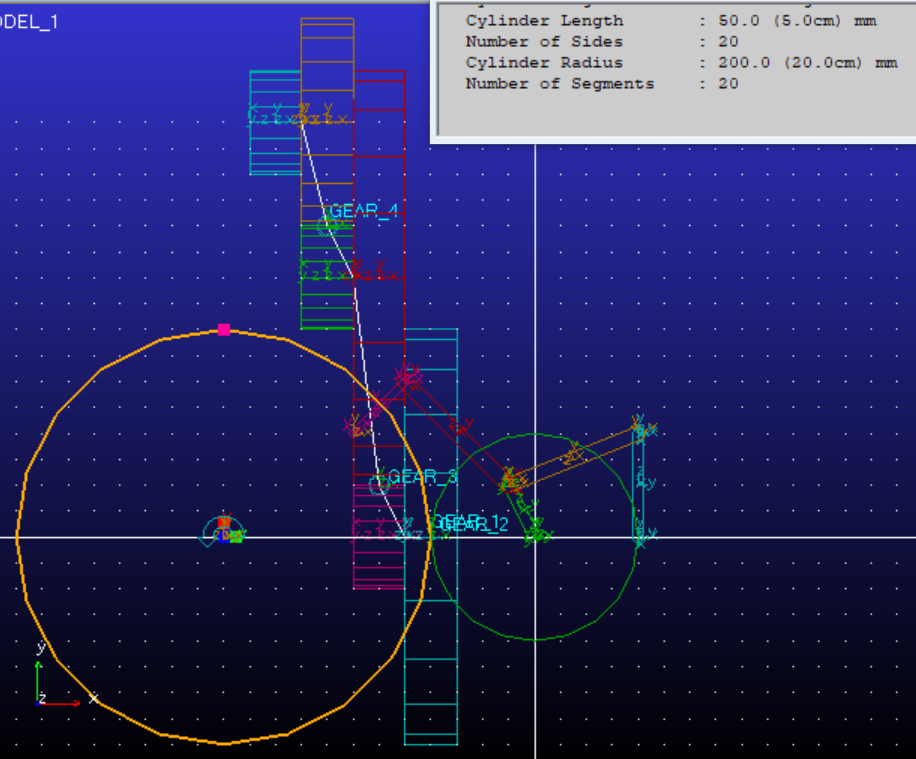
\includegraphics[width=0.9\columnwidth]{Images/dim14.png}
                    \caption{Dimensions of Part 14}
                    \label{fig:dim14}
                \end{figure}

                \begin{figure}[hbt!]
                    \centering
                    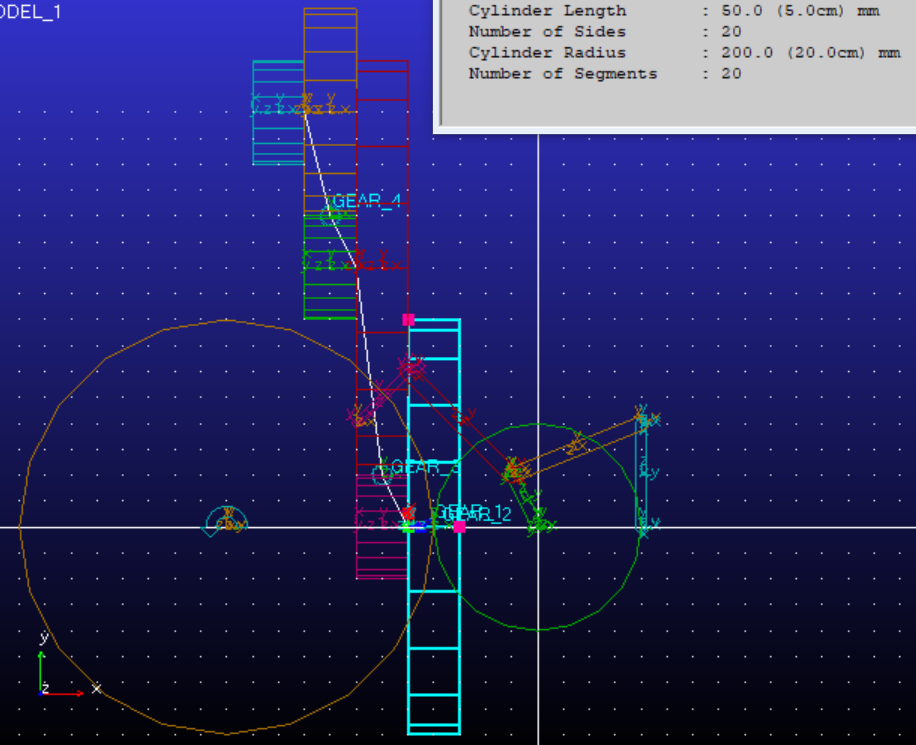
\includegraphics[width=0.9\columnwidth]{Images/dim15.png}
                    \caption{Dimensions of Part 15}
                    \label{fig:dim15}
                \end{figure}

                \begin{figure}[hbt!]
                    \centering
                    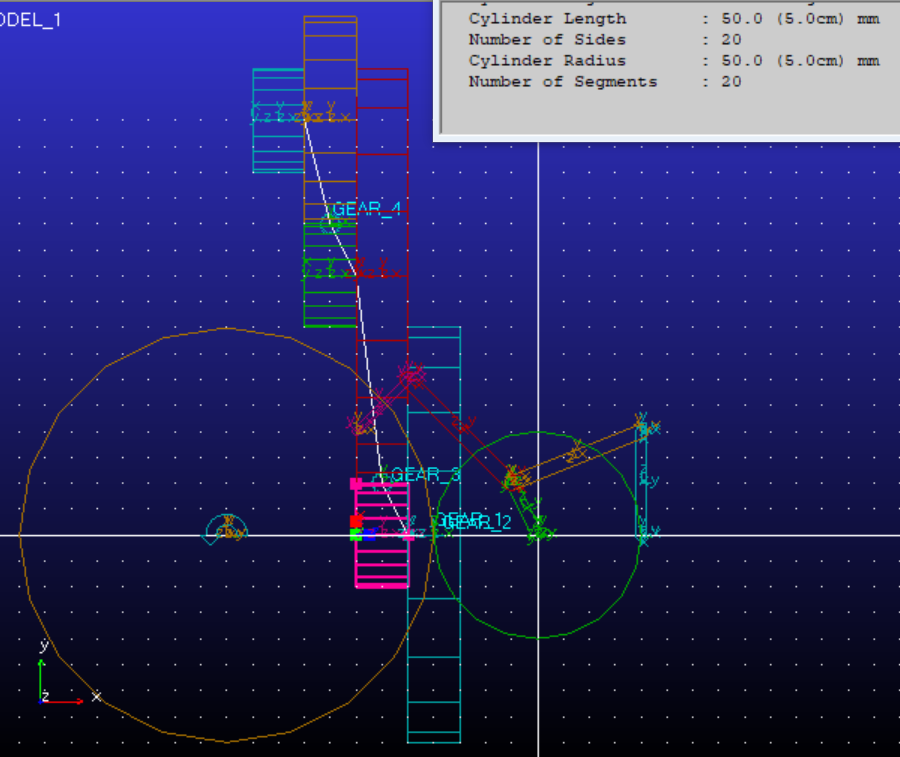
\includegraphics[width=0.9\columnwidth]{Images/dim16.png}
                    \caption{Dimensions of Part 16}
                    \label{fig:dim16}
                \end{figure}

                \begin{figure}[hbt!]
                    \centering
                    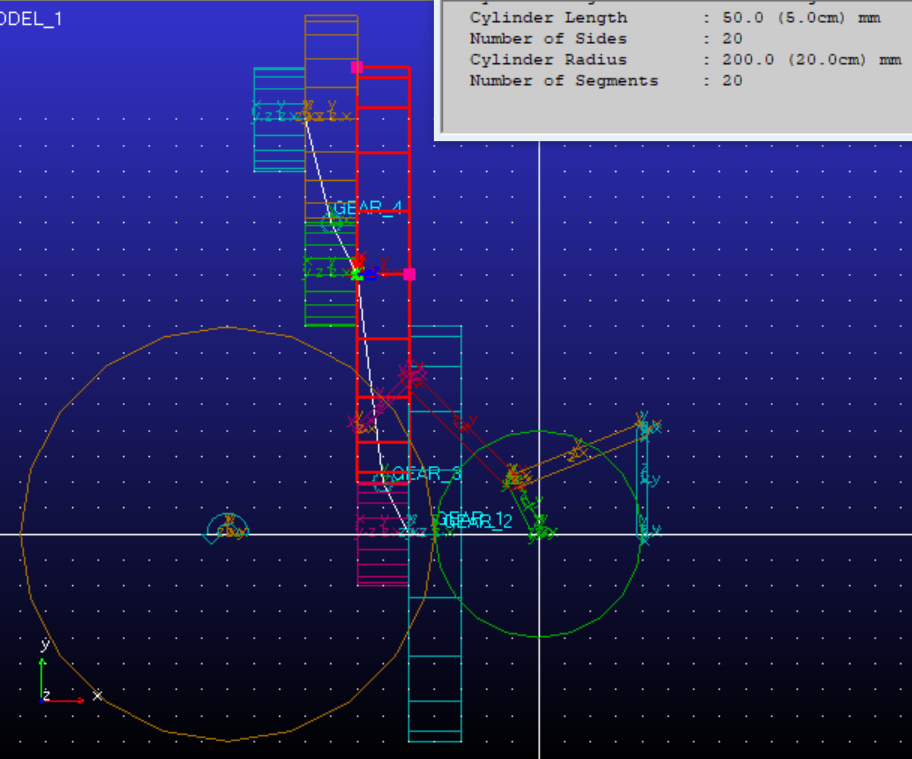
\includegraphics[width=0.9\columnwidth]{Images/dim17.png}
                    \caption{Dimensions of Part 17}
                    \label{fig:dim17}
                \end{figure}

                \begin{figure}[hbt!]
                    \centering
                    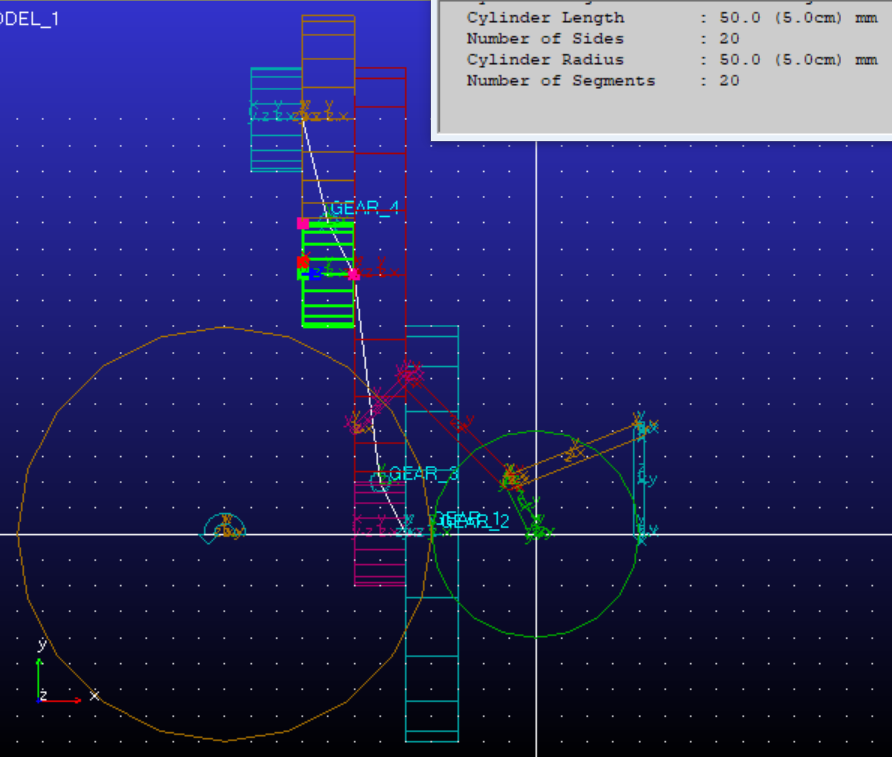
\includegraphics[width=0.9\columnwidth]{Images/dim18.png}
                    \caption{Dimensions of Part 18}
                    \label{fig:dim18}
                \end{figure}

                \begin{figure}[hbt!]
                    \centering
                    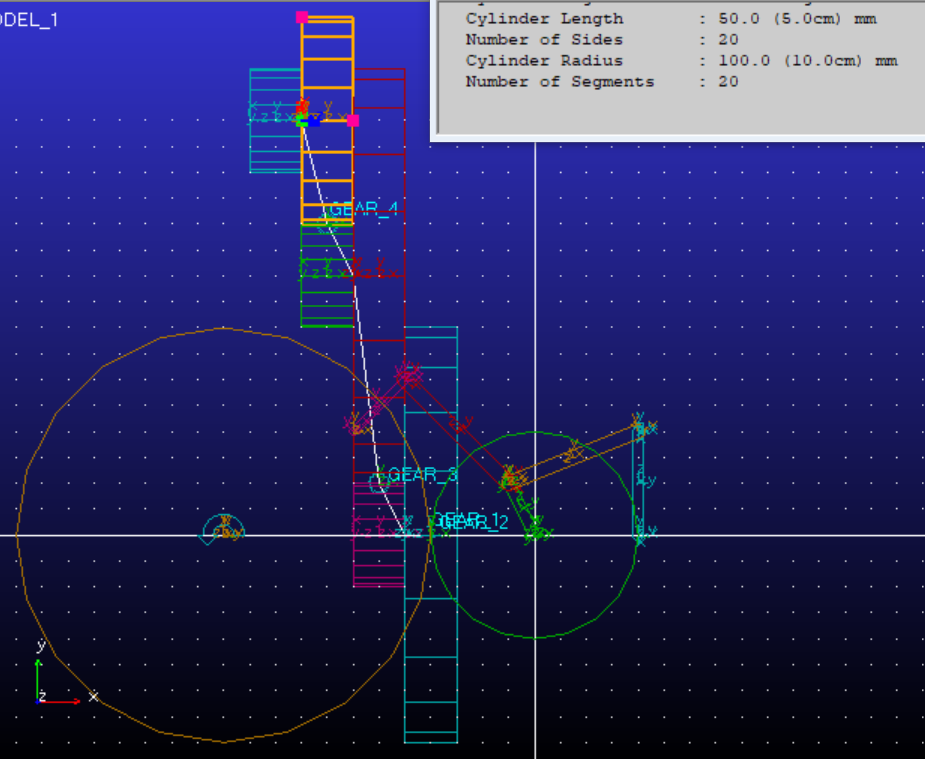
\includegraphics[width=0.9\columnwidth]{Images/dim19.png}
                    \caption{Dimensions of Part 19}
                    \label{fig:dim19}
                \end{figure}

                \begin{figure}[hbt!]
                    \centering
                    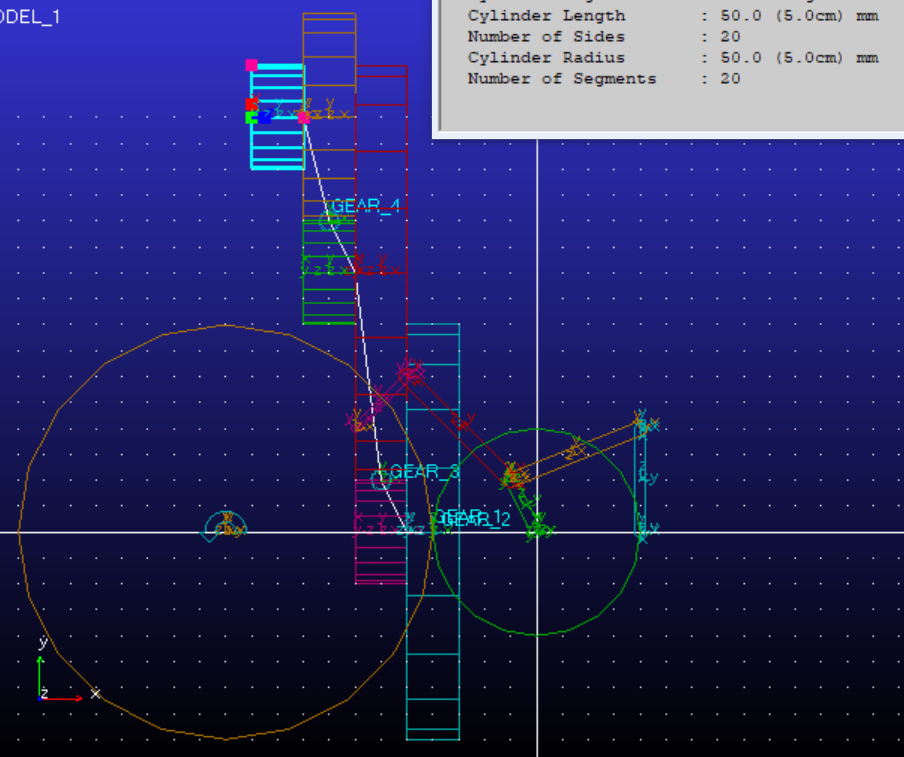
\includegraphics[width=0.9\columnwidth]{Images/dim20.png}
                    \caption{Dimensions of Part 20}
                    \label{fig:dim20}
                \end{figure}

            \subsubsection{Masses of every component}
                \begin{enumerate}
                    \item Part 8: 2.4817759832E-02 kg
                    \item Part 9: 0.1025310773 kg
                    \item Part 10: 0.1025310773 kg
                    \item Part 11: 1.4855713127E-02 kg
                    \item Part 12: 0.118845705 kg
                    \item Part 13: 12.2537821453 kg
                    \item Part 14: 49.0151285813 kg
                    \item Part 15: 49.0151285813 kg
                    \item Part 16: 3.0634455363 kg
                    \item Part 17: 49.0151285813 kg
                    \item Part 18: 3.0634455363 kg
                    \item Part 19: 12.2537821453 kg
                    \item Part 20: 3.0634455363 kg
                \end{enumerate}

            \subsubsection{Moments of inertia of every component}
                \begin{enumerate}
                    \item Part 8: \\ IXX             : 8.6056563943 kg-mm**2 \\
                    IYY             : 8.4571303608 kg-mm**2 \\
                    IZZ             : 0.251933366 kg-mm**2
                    \item Part 9: \\ IXX             : 181.4828571273 kg-mm**2 \\
                    IYY             : 180.3504960967 kg-mm**2 \\
                    IZZ             : 1.9066842627 kg-mm**2
                    \item Part 10: \\ IXX             : 41.0336896795 kg-mm**2 \\
                    IYY             : 40.7776602573 kg-mm**2 \\
                    IZZ             : 0.4311056795 kg-mm**2
                    \item Part 11: \\ IXX             : 7.2538000573 kg-mm**2 \\
                    IYY             : 7.2085400222 kg-mm**2 \\
                    IZZ             : 7.6209437369E-02 kg-mm**2
                    \item Part 12: \\ IXX             : 232.1216018363 kg-mm**2 \\
                    IYY             : 230.6732807113 kg-mm**2 \\
                    IZZ             : 2.4387019949 kg-mm**2
                    \item Part 13: \\ IXX             : 6.1268910727E+04 kg-mm**2 \\
                    IYY             : 3.3187326644E+04 kg-mm**2 \\
                    IZZ             : 3.3187326644E+04 kg-mm**2
                    \item Part 14: \\ IXX             : 9.8030257163E+05 kg-mm**2 \\
                    IYY             : 5.0036277093E+05 kg-mm**2 \\
                    IZZ             : 5.0036277093E+05 kg-mm**2
                    \item Part 15: \\ IXX             : 9.8030257163E+05 kg-mm**2 \\
                    IYY             : 5.0036277093E+05 kg-mm**2 \\
                    IZZ             : 5.0036277093E+05 kg-mm**2
                    \item Part 16: \\ IXX             : 3829.3069204147 kg-mm**2 \\
                    IYY             : 2552.8712802765 kg-mm**2 \\
                    IZZ             : 2552.8712802765 kg-mm**2
                    \item Part 17: \\ IXX             : 9.8030257163E+05 kg-mm**2 \\
                    IYY             : 5.0036277093E+05 kg-mm**2 \\
                    IZZ             : 5.0036277093E+05 kg-mm**2
                    \item Part 18: \\ IXX             : 3829.3069204147 kg-mm**2 \\
                    IYY             : 2552.8712802765 kg-mm**2 \\
                    IZZ             : 2552.8712802765 kg-mm**2
                    \item Part 19: \\ IXX             : 6.1268910727E+04 kg-mm**2 \\
                    IYY             : 3.3187326644E+04 kg-mm**2 \\
                    IZZ             : 3.3187326644E+04 kg-mm**2
                    \item Part 20: \\ IXX             : 3829.3069204147 kg-mm**2 \\
                    IYY             : 2552.8712802765 kg-mm**2 \\
                    IZZ             : 2552.8712802765 kg-mm**2
                \end{enumerate}
                    
        \subsection{Constraints}
            Constrains on the motion of each component. (May require details of the joints.)

            There are mainly three types of joints in my mechanism. Hinge joint, gear joint and locking constraint. The chain drives in the original mechanism have also been modelled as gear joints. That is the reason the gears are so bulky to include the inertial of the shafts as well.

            \begin{enumerate}
                \item Hinge Joint: Between parts 8-9, 9-10, 10-Ground, between all gears and ground.
                \item Gear Joint: Between parts every two cylinder (which is modelled as pitch circle of the gears). Parts 13-14, 14-15, 16-17, 18-19.
                \item Lock joint: Parts 11-12, 12-9, 8-13 and for gear trains 15-16, 17-18, 19-20.
            \end{enumerate}

        \subsection{Motion Transmission}
            \subsubsection{Driving Component}
                The driving component is the engine which goes in the gear box to increase torque and reduce angular velocity which is attached to the gear shown by part 14 which moves at 30 deg per sec of angular velocity.
            
            \subsubsection{Component which gives output of interest}
                The output is given by the links 11 and 12 which are attached to the coupler of the 4-bar mechanism which is responsible for producing the motion to pickup the seedling from the tray and plant it in the ground. \par

                The tray is moved by a chain drive which is attached to the gear/part 20 so that it plants 16 seedlings in a row then changes direction to plant from the next row and so on.

        